\iffalse
\chapter{2022}
\author{AI24BTECH11022}
\section{ce}
\fi

\usetikzlibrary{patterns}
\item You should \rule{1cm}{0.15mm} when to say \rule{1cm}{0.15mm}.\hfill(2022)
\begin{multicols}{2}
\begin{enumerate}
\item no/no
\item no/know
\item know/know
\item know/no
\end{enumerate}
\end{multicols}


\item Two straight lines pass through the origin $\brak{x_{0},y_{0}}=\brak{0,0}$. One of them passes through the point $\brak{x_{1},y_{2}}=\brak{1,3}$ and the other passes through the point $\brak{x_{2},y_{2}}=\brak{1,2}$.

What is the area enclosed between the straight lines in the interval $\sbrak{0,1}$ on the $x-$axis?\hfill(2022)
\begin{multicols}{2}
\begin{enumerate}
\item $0.5$
\item $1.0$
\item $1.5$
\item $2.0$
\end{enumerate}
\end{multicols}


\item If $$p:q=1:2$$ $$q:r=4:3$$ $$r:s=4:5$$ and $u$ is $50\%$ more than $s$, what is the ratio $p:u$?\hfill(2022)
\begin{multicols}{2}
\begin{enumerate}
\item $2:15$
\item $16:15$
\item $1:5$
\item $16:45$
\end{enumerate}
\end{multicols}


\item Given the statements:\\
$P$ is the sister of $Q$.\\
$Q$ is the husband of $R$.\\
$R$ is the mother of $S$.\\
$T$ is the husband of $P$.\\

Based on the above information, $T$ is \rule{1cm}{0.15mm} of $S$.\hfill(2022)
\begin{multicols}{2}
\begin{enumerate}
\item the grandfather
\item an uncle
\item the father
\item a brother
\end{enumerate}
\end{multicols}


\item In the following diagram, the point $R$ is the center of the circle. The lines $PQ$ and $ZV$ are tangential to the circle. The relation among the areas of the squares, $PXWR$, $RUVZ$ and $SPQT$ is\hfill(2022)

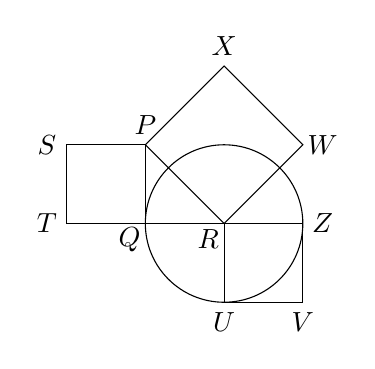
\begin{tikzpicture}
\draw (2,0) rectangle (3,1);
\draw (2,1) circle [radius=1];
\draw (0,1) rectangle (1,2);
\draw (2,1) -- (1,2) -- (2,3) -- (3,2) -- (2,1);
\draw (2,1) -- (1,1);
\node at (2,-0.25) {$U$};
\node at (3,-0.25) {$V$};
\node at (0.8,0.8) {$Q$};
\node at (-0.25,1) {$T$};
\node at (-0.25,2) {$S$};
\node at (1,2.25) {$P$};
\node at (2,3.25) {$X$};
\node at (3.25,2) {$W$};
\node at (3.25,1) {$Z$};
\node at (1.8,0.8) {$R$};
\end{tikzpicture}

\begin{enumerate}
\item Area of $SPQT=$Area of $RUVZ=$Area of $PXWR$
\item Area of $SPQT=$Area of $PXWR-$Area of $RUVZ$
\item Area of $PXWR=$Area of $SPQT-$Area of $RUVZ$
\item Area of $PXWR=$Area of $RUVZ-$Area of $SPQT$
\end{enumerate}


\item Healthy eating is a critical component of healthy aging. When should one start eating healthy? It turns out that it is never too early. For example, babies who start eating healthy in the first year are more likely to have better overall health as they get older.

Which one of the following is the CORRECT logical inference based on the information in the above passage?\hfill(2022)
\begin{enumerate}
\item Healthy eating is important for those with good health conditions, but not for others
\item Eating healthy can be started at any age, earlier the better
\item Eating healthy and better overall health are more correlated at a young age, but not older age
\item Healthy eating is more important for adults than kids
\end{enumerate}


\item $P$ invested $5000$ rupees per month for $6$ months of a year and $Q$ invested $x$ rupees per month for $8$ months of the year in a partnership business. The profit is shared in proportion to the total investment made in that year.

If at the end of that investment year, $Q$ receives $\frac{4}{9}$ of the total profit, what is the value of $x$ (in rupees)?\hfill(2022)
\begin{multicols}{2}
\begin{enumerate}
\item $2500$
\item $3000$
\item $4687$
\item $8437$
\end{enumerate}
\end{multicols}


\item 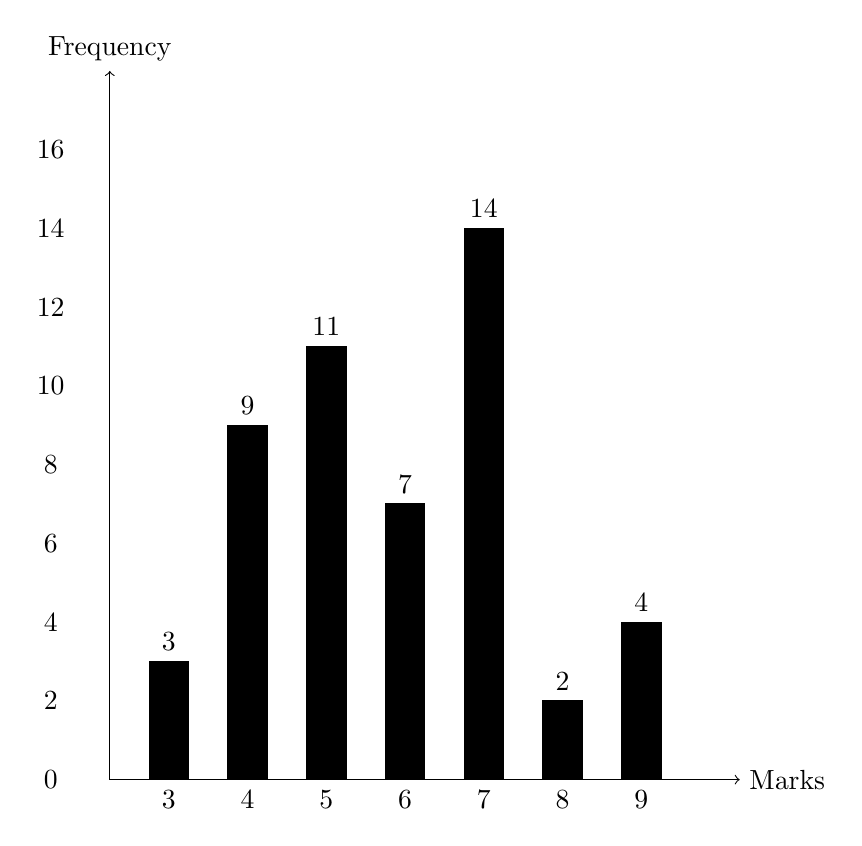
\begin{tikzpicture}
\draw[->] (0.5,0) -- (8.5,0) node[right] {Marks};
\draw[->] (0.5,0) -- (0.5,9) node[above] {Frequency};
\draw[fill=black] (1,0) rectangle (1.5,1.5);
\draw[fill=black] (2,0) rectangle (2.5,4.5);
\draw[fill=black] (3,0) rectangle (3.5,5.5);
\draw[fill=black] (4,0) rectangle (4.5,3.5);
\draw[fill=black] (5,0) rectangle (5.5,7);
\draw[fill=black] (6,0) rectangle (6.5,1);
\draw[fill=black] (7,0) rectangle (7.5,2);
\node at (1.25,1.75) {3};
\node at (2.25,4.75) {9};
\node at (3.25,5.75) {11};
\node at (4.25,3.75) {7};
\node at (5.25,7.25) {14};
\node at (6.25,1.25) {2};
\node at (7.25,2.25) {4};
\node at (1.25, -0.25) {3};
\node at (2.25, -0.25) {4};
\node at (3.25, -0.25) {5};
\node at (4.25, -0.25) {6};
\node at (5.25, -0.25) {7};
\node at (6.25, -0.25) {8};
\node at (7.25, -0.25) {9};
\foreach \y in {0,2,4,6,8,10,12,14,16} {
\node at (-0.25, \y/2) {\y};
}
\end{tikzpicture}

The above frequency chart shows the frequency distribution of marks obtained by a set of students in an exam.

From the data presented above, which one of the following is CORRECT?\hfill(2022)
\begin{multicols}{2}
\begin{enumerate}
\item mean$>$mode$>$median
\item mode$>$median$>$mean
\item mode$>$mean$>$median
\item median$>$mode$>$mean
\end{enumerate}
\end{multicols}


\item In the square grid shown on the left, a person standing at $P2$ position is required to move to $P5$ position.

The only movement allowed for a step involves, "two moves along one direction followed by one move in a perpendicular direction". The permissible directions for movement are shown as dotted arrows in the right.

For example, a person at a given position $Y$ can move only to the positions marked $X$ on the right.

Without occupying any of the shaded squares at the end of each step, the minimum number of steps required to go from $P2$ to $P5$ is\hfill(2022)

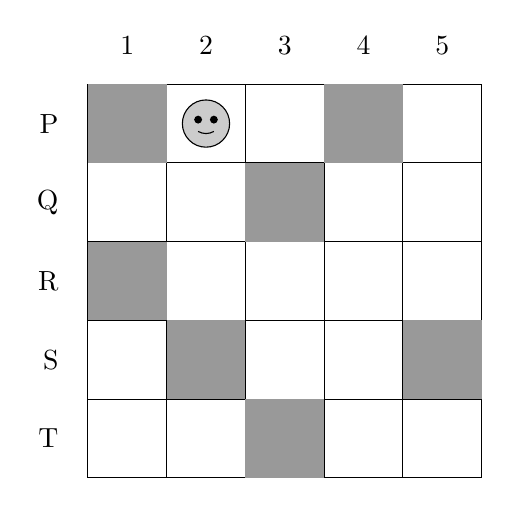
\begin{tikzpicture}
\draw[step=1cm,black] (0,0) grid (5,5);
\fill[gray!80] (0,4) rectangle (1,5);
\fill[gray!80] (3,4) rectangle (4,5);
\fill[gray!80] (2,3) rectangle (3,4);
\fill[gray!80] (0,2) rectangle (1,3);
\fill[gray!80] (1,1) rectangle (2,2);
\fill[gray!80] (4,1) rectangle (5,2);
\fill[gray!80] (2,0) rectangle (3,1);
\node[left] at (-0.25,4.5) {P};
\node[left] at (-0.25,3.5) {Q};
\node[left] at (-0.25,2.5) {R};
\node[left] at (-0.25,1.5) {S};
\node[left] at (-0.25,0.5) {T};
\node[above] at (0.5,5.25) {1};
\node[above] at (1.5,5.25) {2};
\node[above] at (2.5,5.25) {3};
\node[above] at (3.5,5.25) {4};
\node[above] at (4.5,5.25) {5};
\begin{scope}[shift={(1.5,4.5)}]
\draw[fill=gray!40] (0,0) circle (0.3);
\fill (-.1,.05) circle (0.05);
\fill (.1,.05) circle (0.05);
\draw[black] (-.1,-.1) arc (-120:-60:0.2);
\end{scope}
\end{tikzpicture}

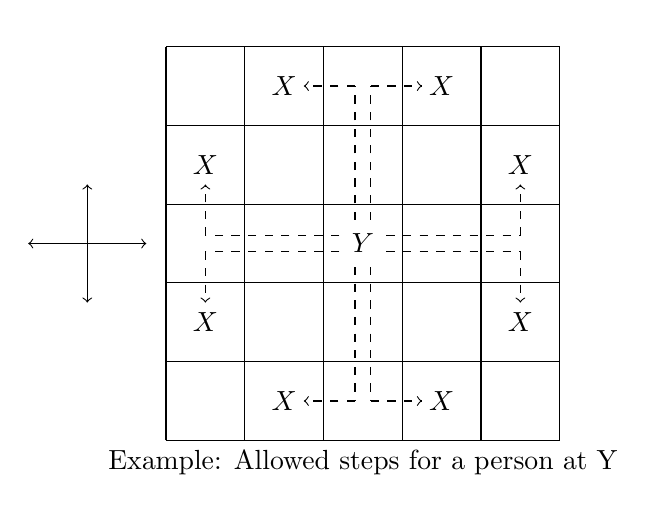
\begin{tikzpicture}
\draw[<->] (-1.75,2.5) -- (-0.25,2.5);
\draw[<->] (-1,1.75) -- (-1,3.25);
\draw[step=1cm] (0,0) grid (5,5);
\node at (2.5,2.5) {$Y$};
\node at (0.5,1.5) {$X$};
\node at (0.5,3.5) {$X$};
\node at (1.5,0.5) {$X$};
\node at (1.5,4.5) {$X$};
\node at (3.5,0.5) {$X$};
\node at (3.5,4.5) {$X$};
\node at (4.5,1.5) {$X$};
\node at (4.5,3.5) {$X$};
\draw[dashed] (2.2,2.4) -- (0.5,2.4);
\draw[dashed] (2.8,2.4) -- (4.5,2.4);
\draw[dashed] (2.2,2.6) -- (0.5,2.6);
\draw[dashed] (2.8,2.6) -- (4.5,2.6);
\draw[dashed] (2.4,2.2) -- (2.4,0.5);
\draw[dashed] (2.4,2.8) -- (2.4,4.5);
\draw[dashed] (2.6,2.2) -- (2.6,0.5);
\draw[dashed] (2.6,2.8) -- (2.6,4.5);\
\draw[dashed,->] (0.5,2.4) -- (0.5,1.75);
\draw[dashed,->] (0.5,2.6) -- (0.5,3.25);
\draw[dashed,->] (4.5,2.4) -- (4.5,1.75);
\draw[dashed,->] (4.5,2.6) -- (4.5,3.25);
\draw[dashed,->] (2.4,0.5) -- (1.75,0.5);
\draw[dashed,->] (2.6,0.5) -- (3.25,0.5);
\draw[dashed,->] (2.4,4.5) -- (1.75,4.5);
\draw[dashed,->] (2.6,4.5) -- (3.25,4.5);
\node[below] at (2.5,0) {Example: Allowed steps for a person at Y};
\node[above] at (2.5,5) {};
\end{tikzpicture}
\begin{multicols}{2}
\begin{enumerate}
\item $4$
\item $5$
\item $6$
\item $7$
\end{enumerate}
\end{multicols}


\item 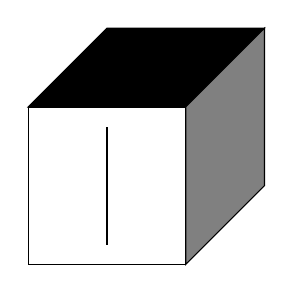
\begin{tikzpicture}
\coordinate (A) at (0,0);
\coordinate (B) at (2,0);
\coordinate (C) at (2,2);
\coordinate (D) at (0,2);
\coordinate (E) at (1,1);
\coordinate (F) at (3,1);
\coordinate (G) at (3,3);
\coordinate (H) at (1,3);
\fill[white] (A) -- (B) -- (C) -- (D) -- cycle;
\draw (A) -- (B) -- (C) -- (D) -- cycle;
\fill[black] (D) -- (C) -- (G) -- (H) -- cycle;
\draw (D) -- (C) -- (G) -- (H) -- cycle;
\fill[gray] (B) -- (C) -- (G) -- (F) -- cycle;
\draw (B) -- (C) -- (G) -- (F) -- cycle;
\draw (1,0.25) -- (1,1.75);
\end{tikzpicture}

Consider a cube made by folding a single sheet of paper of appropriate shape. The interior faces of the cube are all blank. However, the exterior faces that are not visible in the above view may not be blank.

Which one of the following represents a possible unfolding of the cube?\hfill(2022)
\begin{multicols}{2}
\begin{enumerate}
\item 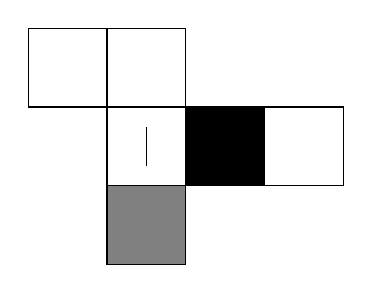
\begin{tikzpicture}
\draw (0,2) rectangle (1,3);
\draw (1,2) rectangle (2,3);
\draw (1,1) rectangle (2,2);
\draw (1.5,1.25) -- (1.5,1.75);
\fill[black] (2,1) rectangle (3,2);
\draw (2,1) rectangle (3,2);
\draw (3,1) rectangle (4,2);
\fill[gray] (1,0) rectangle (2,1);
\draw (1,0) rectangle (2,1);
\end{tikzpicture}
\item 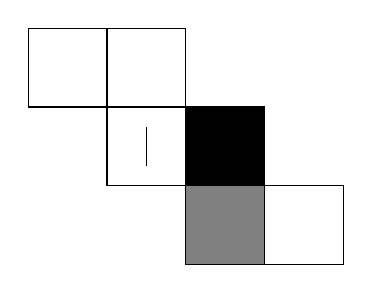
\begin{tikzpicture}
\draw (0,2) rectangle (1,3);
\draw (1,2) rectangle (2,3);
\draw (1,1) rectangle (2,2);
\draw (1.5,1.25) -- (1.5,1.75);
\fill[black] (2,1) rectangle (3,2);
\draw (2,1) rectangle (3,2);
\fill[gray] (2,0) rectangle (3,1);
\draw (2,0) rectangle (3,1);
\draw (3,0) rectangle (4,1);
\end{tikzpicture}
\item 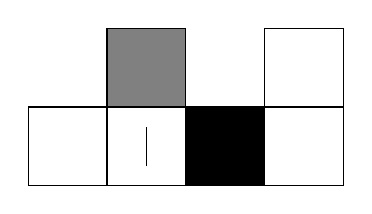
\begin{tikzpicture}
\draw (0,1) rectangle (1,2);
\draw (1,1) rectangle (2,2);
\draw (1.5,1.25) -- (1.5,1.75);
\fill[gray] (1,2) rectangle (2,3);
\draw (1,2) rectangle (2,3);
\fill[black] (2,1) rectangle (3,2);
\draw (2,1) rectangle (3,2);
\draw (3,1) rectangle (4,2);
\draw (3,2) rectangle (4,3);
\end{tikzpicture}
\item 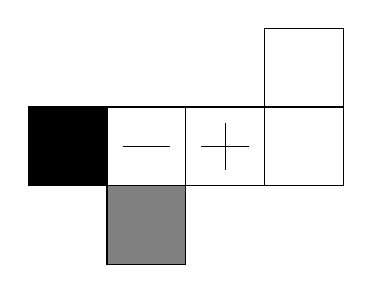
\begin{tikzpicture}
\fill[black] (0,1) rectangle (1,2);
\draw (0,1) rectangle (1,2);
\draw (1,1) rectangle (2,2);
\draw (1.2,1.5) -- (1.8,1.5);
\draw (2,1) rectangle (3,2);
\draw (2.2,1.5) -- (2.8,1.5);line
\draw (2.5,1.2) -- (2.5,1.8);
\draw (3,1) rectangle (4,2);
\draw (3,2) rectangle (4,3);
\fill[gray] (1,0) rectangle (2,1);
\draw (1,0) rectangle (2,1);
\end{tikzpicture}
\end{enumerate}
\end{multicols}


\item Consider the following expression:

$$z=\sin{\brak{y+it}}+\cos{\brak{y-it}}$$ where $z$, $y$ and $t$ are variables, and $i=\sqrt{-1}$ is a complex number. The partial differential equation derived from the above expression is\hfill(2022)
\begin{multicols}{2}
\begin{enumerate}
\item $\frac{\partial^{2}z}{\partial t^{2}}+\frac{\partial^{2}z}{\partial y^{2}}=0$
\item $\frac{\partial^{2}z}{\partial t^{2}}-\frac{\partial^{2}z}{\partial y^{2}}=0$
\item $\frac{\partial z}{\partial t}-i\frac{\partial z}{\partial y}=0$
\item $\frac{\partial z}{\partial t}+i\frac{\partial z}{\partial y}=0$
\end{enumerate}
\end{multicols}


\item For the equation $$\frac{d^{3}y}{dx^{3}}+x\brak{\frac{dy}{dx}}^{\frac{3}{2}}+x^{2}y=0$$ the correct description is\hfill(2022)
\begin{enumerate}
\item an ordinary differential equation of order $3$ and degree $2$.
\item an ordinary differential equation of order $3$ and degree $3$.
\item an ordinary differential equation of order $2$ and degree $3$.
\item an ordinary differential equation of order $3$ and degree $\frac{3}{2}$.
\end{enumerate}

\item The hoop stress at a point on the surface of a thin cylindrical pressure vessel is computed to be $30.0MPa$. The value of maximum shear stress at this point is\hfill(2022)
\begin{multicols}{2}
\begin{enumerate}
\item $7.5MPa$
\item $15.0MPa$
\item $30.0MPa$
\item $22.5MPa$
\end{enumerate}
\end{multicols}